\chapter{Flavour physics and CP symmetry violation}
This chapter explores the theoretical framework for the rest of the thesis.
Section \ref{sec:sm} will provide a basic introduction to the Standard Model of Particle Physics and flavour physics in particular;
Section \ref{sec:discrete} will delve into the inner workings of discrete symmetries in quantum physics;
Section \ref{sec:edms} will discuss the relevance of electromagnetic dipole moments of elementary particles as a test for CP violation and CPT symmetry;
finally, Section \ref{sec:lambda} will introduce the main topic of the thesis, the study of dipole moments of the $\Lambda$ baryon.

\section{The Standard Model of Particle Physics}
\label{sec:sm}
Ever since Democritus' philosophy of atomism, one of the driving desires behind mankind's advancements in the fields of natural science has been to reduce reality to its basic components.
While one can convincingly argue that we may never fully understand what has come to be known as the quantum world, the Standard Model of Particle Physics (Standard Model, or SM, for short) is as close as physics has to offer to a comprehensive theory of the building blocks of matter and energy.

[... Qualcosa sulle previsioni sperimentali confermate.]

While the Standard Model is a self-consistent theory tested to a high degree of precision, it would be a serious mistake to call it \textit{complete}, even if only for the three fundamental forces it covers.
Many experimental evidences, some of which will be discussed in the following pages, have already opened cracks in the model, and many more are likely to emerge in the future;
one of the recurring topics of this chapter will thus be the need for physics Beyond the Standard Model (BSM).

\subsection{Elementary particles}
\begin{figure}[t!]
	\centering
	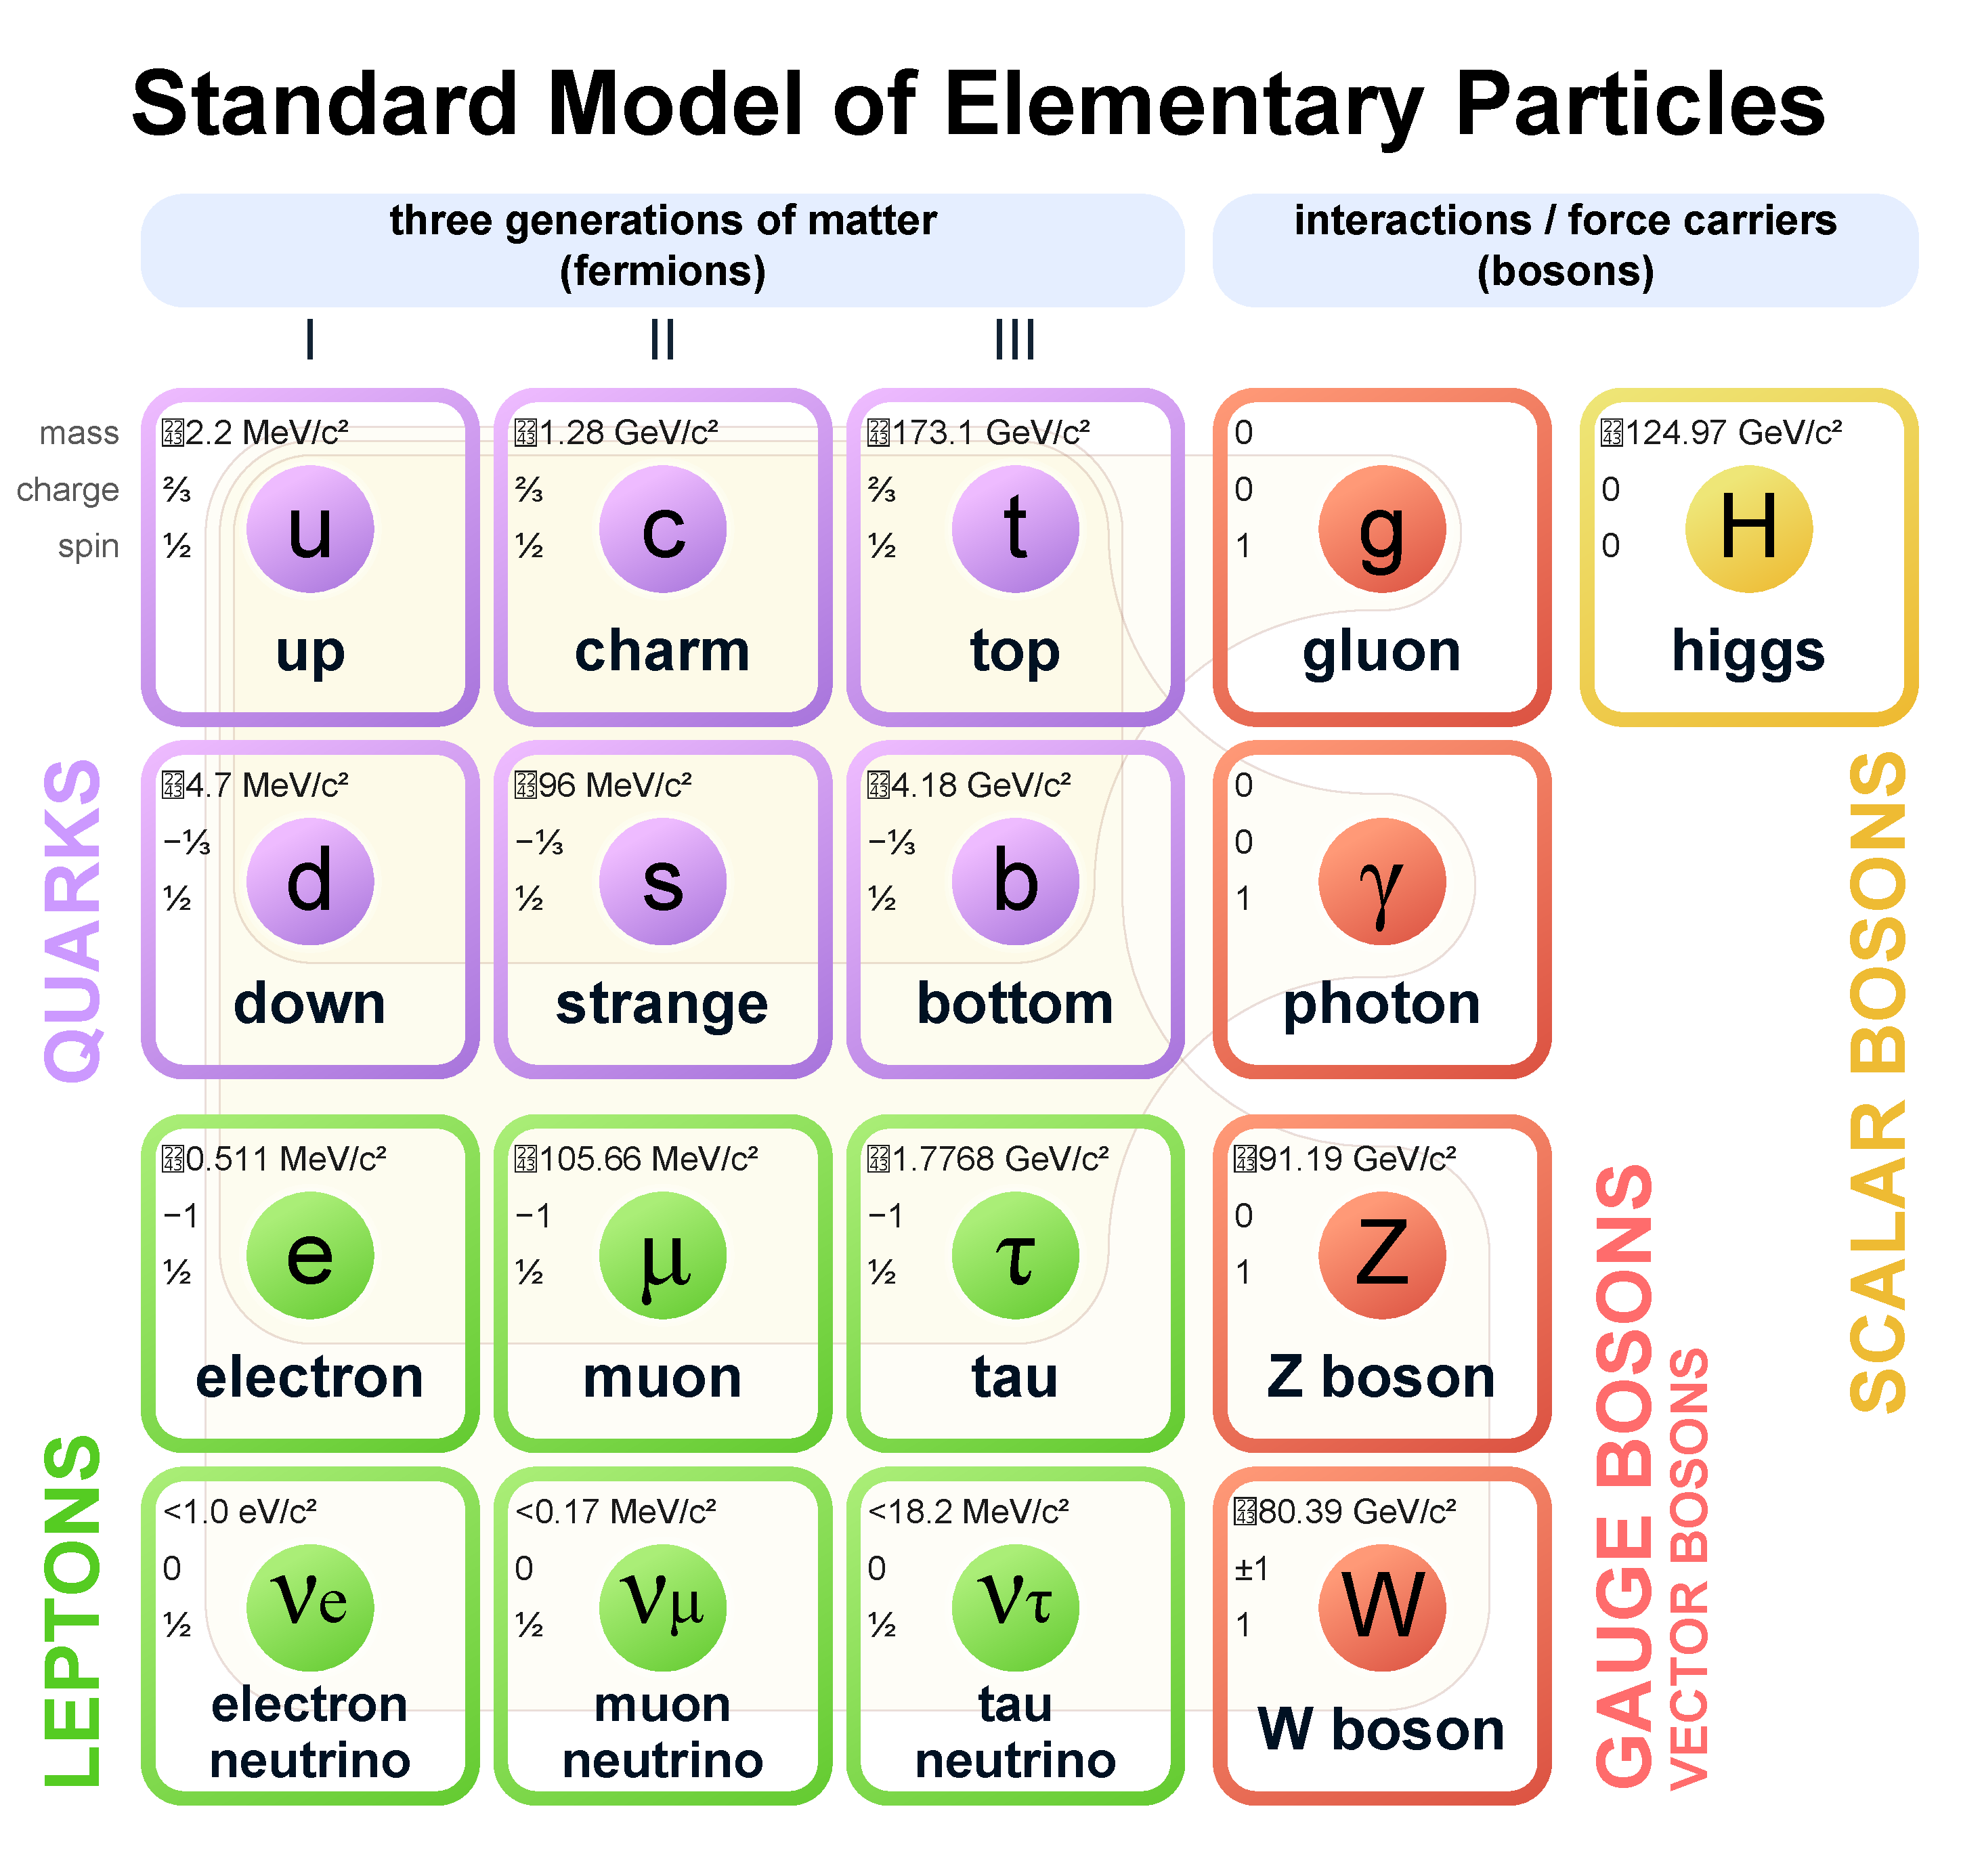
\includegraphics[scale=0.15]{graphics/01-standard_model/Standard_Model_of_Elementary_Particles.pdf}
	\caption[Currently known Standard Model elementary particles.]{The seventeen currently known elementary particles of the Standard Model. Antiparticles are not depicted.}
	\label{fig:particle_zoo}
\end{figure}

Intuitively, a particle is said to be \textit{elementary} when no substructure can be probed. 
A century of efforts in the fields of nuclear, quantum, and high energy physics has whittled down the spectrum of matter to just seventeen unique fundamental particles, colloquially known as the \textit{particle zoo} and depicted in Figure \ref{fig:particle_zoo}.

Each particle is joined by an \textit{antimatter particle} (\textit{antiparticle} for short), a companion of opposite charge identified by the prefix \textit{anti-}, e.g. antimuon for the muon; the only exception to this naming convention is the electron, whose antiparticle, for historical reasons, is known as positron.
While often omitted for the sake of brevity, antiparticles are elementary particles in every respect, distinct from their partners (bar the neutral gauge bosons, which are their own antiparticles) and related to them through the transformation of charge conjugation (see Section \ref{sec:C-symmetry}).

\subsubsection{Leptons}
Leptons are fermions (half-integer spin particles) not sensitive to the strong nuclear interaction.
There are currently six \textit{flavours} of leptons grouped in three generations: each generation comprises a \textit{charged} lepton (electron, muon, tauon) and a \textit{neutral} lepton (electron neutrino, muon neutrino, tauon neutrino).

All charged leptons have a charge of $-e$, where $e$ is defined as the \textit{elementary positive charge}, and their mass ranges from $\approx \SI{0.5}{MeV}$ for the electron to over $\SI{1.7}{GeV}$ for the tauon.
By contrast, as the names suggest, all neutrinos are electrically neutral and are assumed massless in the Standard Model\footnote{The observation of flavour oscillation in solar neutrinos shows that neutrinos do in fact have non-zero, albeit very small, mass.}; this implies that their only meaningful interactions happen through the weak nuclear force, which grants them their characteristic evasiveness to most particle detectors.


\subsubsection{Quarks}
Much like leptons, quarks are also fermions existing in three generations. The main difference from the former category is that quarks, besides interacting through weak and electromagnetic forces, are also susceptible to the strong nuclear forces; this allows them to bind together in composite states known as \textit{hadrons}, which are classified as \textit{baryons} (states of three quarks) and \textit{mesons} (states of one quark and one antiquark)\footnote{As recently as 2003, evidence has surfaced for the existence of exotic baryons composed of four (\textit{tetraquarks}) and five quarks (\textit{pentaquarks}).}.

Quarks can be classified as \textit{up-type} (up, charm and top quarks) and \textit{down-type} (down, strange and bottom quarks): up-type quarks have a fractionary charge of $+\frac{2}{3} e$, whereas down-type quarks have a charge of $-\frac{1}{3} e$. All quarks also have one of three \textit{color} charges (red, green or blue), while antiquarks similarly have one of three \textit{anti-color} charges (antired, antigreen or antiblue). A combination of all three colors/anti-colors or a combination of a color and its matching anticolor produces \textit{colorless} particles, a property of all observed quark composite states.

Unlike leptons, quarks are impossible to observe directly: according to the phenomenon of \textit{color confinement}, the energy of the interaction field between two color charges being pulled apart increases with their distance until it becomes high enough to create a quark-antiquark pair.
This process of \textit{fragmentation} develops many times over in such a way that the final observable state is entirely composed of colorless particles.
For this reason, high energy physics experiments such as LHCb do not detect free quarks, instead observing cone-shaped streams of hadrons known as \textit{hadronic jets}.

\subsubsection{Gauge bosons and fundamental interactions}
In quantum field theory, the interaction between two fields is implemented through the exchange of an intermediary particle known as \textit{force carrier}.
In the Standard Model all force carriers are vector (spin $1$) bosons known as \textit{gauge bosons}, the name being owed to the \textit{gauge principle} used to introduce them: the localization of a global continuous symmetry group provides the free fermion Lagrangians with interaction terms with the proviso that one or more bosonic fields are introduced.

%The fundamental forces driving the interactions between elementary particles are introduced in the Standard Model via the so-called \textit{gauge principle}, which adds an interaction term to the free Lagrangian as a result of the localization of a global continuous symmetry group; accordingly, the related force carriers are known as \textit{gauge bosons}.

The gauge principle accounts for the implementation of three fundamental interactions along with their gauge bosons: 
the \textit{strong nuclear force} with its massless gluon, responsible for the binding of both quarks inside baryons and nucleons inside atomic nuclei; the \textit{electromagnetic force} mediated by the massless photon, the importance of which should be known from everyday life; and the \textit{weak nuclear force} with two massive $W^\pm$ and $Z$ bosons, the source of many subnuclear processes such as $\beta$ radioactivity.

The latter two forces share a unified description in the Glashow-Weinberg-Salam theory as a single \textit{electroweak interaction} and are introduced via localization of a $\text{SU(2)}_L \otimes \text{U(1)}_Y$ symmetry group, the first related to the conservation of weak isospin in left-handed chirality states and the second to the conservation of hypercharge.
Quantum chromodynamics (QCD), the theory of the strong nuclear force, is based on a separate $\text{SU(3)}_C$ symmetry acting on the three-dimensional space of color charges.

There are no gauge bosons nor gauge theories associated to the fourth known fundamental force, gravity.
Since every attempt to reconcile the general theory of relativity with quantum mechanics has failed so far, gravity is presently excluded from the Standard Model;
this doesn't affect SM predictions at the subatomic level on account of the remarkably low intensity of said force, over 30 orders of magnitude lower than the weak interaction.

\subsubsection{The Higgs boson}
The Higgs boson is one of the latest additions to the Standard Model, being proposed in 1964 and observed by the ATLAS and CMS collaborations in 2012.
Its introduction solved perhaps the most insidious SM shortcoming at the time: gauge theories, which the model was built on, only worked under the assumption that all particles involved were massless, whereas the local invariance would fall apart (\textit{gauge breaking}) when adding a free mass term.

By contrast, the Higgs field accounts for mass generation of the weak bosons $W^\pm$ and $Z$ via the Brout-Englert-Higgs mechanism resulting from the spontaneous electroweak symmetry breaking;
elementary fermions also gain mass through a distinct, Yukawa-like interaction with the field.

\subsection{Flavour physics} \label{sec:flavour-physics}
A reader unfamiliar with SM terminology may find amusing the use of the word \textit{flavour} to refer to what have been so far presented as different kinds of particles altogether.
However quirky, the lexical choice highlights a defining feature: flavour, much like the degree of sweetness in a recipe, can change.

As often happens in particle physics, the rules are somewhat easier for leptons. For a given generation $\ell = (e,\mu,\tau)$, one can define a \textit{lepton family number} $L_\ell$ as the difference between the number of particles and antiparticles of said generation, charged leptons and neutrinos alike:
\begin{equation}
L_\ell
\coloneqq
n(\ell^-) - n(\ell^+)
+
n(\nu_\ell) - n(\bar{\nu}_\ell).
\end{equation}
For all three generations, $L_\ell$ is conserved in every interaction except neutrino oscillations.

Quarks are not as straightforward.
A similarly defined quark flavour number, such as the so-called \textit{topness} (or \textit{truth})
\begin{equation}
T
\coloneqq
n(t) - n(\bar{t}),
\end{equation}
is preserved through EM and strong interactions, but can change when the state undergoes a \textit{weak charged interaction}, i.e. a weak interaction mediated by the charged gauge bosons $W^\pm$. In fact, one finds that weak interactions for quarks can be accurately described if we assume that the weak eigenstates $(d',s',b')$ of down-type quarks, i.e. the weak isospin doublet partners to up-type quarks, are related to the free mass eigenstates $(d,s,b)$ through a rotation:
\begin{equation}
	\begin{pmatrix}
		d' \\
		s' \\
		b'
	\end{pmatrix}
	=
	\begin{pmatrix}
		V_{ud} & V_{us} & V_{ub} \\
		V_{cd} & V_{cs} & V_{cb} \\
		V_{td} & V_{ts} & V_{tb}
	\end{pmatrix}
	\begin{pmatrix}
		d \\
		s \\
		b
	\end{pmatrix}.
	\label{eq:CKM-matrix-mixing}
\end{equation}
In this notation, the probability for a quark of flavour $i$ to change into a quark of flavour $j$ as a result of a weak charged interaction is proportional to ${\left| V_{ij} \right|}^2$.

The unitary rotation matrix is known as the Cabibbo-Kobayashi-Maskawa (CKM) matrix $V_\text{CKM}$. The moduli of its components up to the third decimal place, according to the most recent estimates, are
\begin{equation}
	\begin{pmatrix}
		\left|V_{ud}\right| & \left|V_{us}\right| & \left|V_{ub}\right| \\
		\left|V_{cd}\right| & \left|V_{cs}\right| & \left|V_{cb}\right| \\
		\left|V_{td}\right| & \left|V_{ts}\right| & \left|V_{tb}\right|
	\end{pmatrix}
	\approx 
	\begin{pmatrix}
		0.974 & 0.224 & 0.004 \\
		0.221 & 0.987 & 0.041 \\
		0.008 & 0.039 & 1.013
	\end{pmatrix}.
	\label{eq:CKM-matrix-numerical}
\end{equation}

A full definition of the CKM matrix requires four independent parameters.
Particularly useful for the following sections is the standard parameterization with three angles $\theta_{12}$, $\theta_{23}$, $\theta_{13}$, expressing the mixing between different quark generations, and a complex phase $\delta_{13}$.
Defining $s_{ik} \coloneqq \sin\theta_{ik}$ and $c_{ik} \coloneqq \cos\theta_{ik}$, $V_\text{CKM}$ can be written as
\begin{equation}
	V_\text{CKM}
	=
	\begin{pmatrix}
		c_{12} c_{13}
		&
		s_{12} c_{13}
		&
		s_{13} e^{-i\delta_{13}}
		\\
		- s_{12} c_{23} - c_{12} s_{23} s_{13} e^{i\delta_{13}}
		&
		c_{12} c_{23} - s_{12} s_{23} s_{13} e^{i\delta_{13}}
		&
		s_{23} c_{13}
		\\
		s_{12} s_{23} - c_{12} c_{23} s_{13} e^{i\delta_{13}}
		&
		-c_{12} s_{23} - s_{12} c_{23} s_{13} e^{i\delta_{13}}
		&
		c_{23} c_{13}
	\end{pmatrix}	
	\label{eq:CKM-matrix-parameterization}
\end{equation}

The phase $\delta_{13}$ is known as the CP-violating phase. To fully understand what it means and its role in particle physics, however, a digression into discrete symmetries is needed.

\section{Discrete symmetries and CP violation}
\label{sec:discrete}
In quantum mechanics, a system described by an Hamiltonian $\hat{\mathcal{H}}$ is \textit{symmetric} under a transformation $\hat{S}$ if the two operators commute, i.e.
\begin{equation}
\left[ \hat{\mathcal{H}}, \hat{S} \right] = 0.
\end{equation}
Symmetries are of great relevance in physics on account of Noether's theorem, which establishes a relationship between the \textit{continuous} symmetry of a system and a corresponding conservation law;
the emphasis is on the requirement of continuity, meaning the related transformation changes the system <<in a smooth way>>, much like a rotation does.
An example of this principle has already been presented earlier in this thesis:
the three symmetry groups employed in SM gauge theories all imply the conservation of a specific charge, be it weak isospin, hypercharge, or color.

By contrast, this section will delve into \textit{discrete} symmetries, which do not share said <<smoothness>> property.
The absence of a Noether-like theorem for this class of transformations does not detract from their importance in physics:
as will be shown, the three symmetries we'll focus on have a remarkable influence on many fields of study.

\subsection{Parity inversion}
By definition, the \textit{parity inversion} (or simply \textit{parity}) transformation $\hat{P}$ flips the sign of the three spatial coordinates:
\begin{equation}
	\hat{P} : \begin{pmatrix}
		x \\ y \\ z
	\end{pmatrix}
	\rightarrow
	\begin{pmatrix}
		-x \\ -y \\ -z
	\end{pmatrix}.
\end{equation}
Its action on a quantum $\ket{\psi(\vec{x},t)}$ is therefore
\begin{equation}
	\hat{P} \ket{\psi(\vec{x},t)} = \ket{\psi(-\vec{x},t)}.
\end{equation}

More interestingly, for parity eigenstates (known as \textit{parity-defined} states) a parity quantum number can be introduced;
such states may have a \textit{P-parity} eigenvalue $\eta_p = +1$ (parity-even states) or $\eta_p = -1$ (parity-odd states).
Since by definition $\hat{P}^2 = \mathds{1}$, where $\mathds{1}$ is the identity operator, these are the only two allowed P-parity values.

A similarly dichotomous behaviour is observed on both scalar and vector quantities commonly used in classical physics, such as momenta and electromagnetic fields.
Parity-even scalar quantities are called \textit{true scalars} or just \textit{scalars} (e.g. energy), whereas parity-odd ones are called \textit{pseudoscalars} (e.g. helicity).
The same distinction is present for vector quantities, which are either \textit{polar vectors} (e.g. angular momentum) or \textit{axial vectors} (e.g. linear momentum).

As far as is currently known, gravity, electromagnetic and strong nuclear interactions conserve parity.
The same cannot be said for the weak interaction, the P-violating properties of which were first proven in the 1956 Wu experiment on the $^{60}\text{Co}$ $\beta^-$ decay. 

\subsection{Charge conjugation}
\label{sec:C-symmetry}
The transformation of \textit{charge conjugation} $\hat{C}$ changes the sign of all electric charges:
\begin{equation}
	\hat{C} : q \rightarrow -q.
\end{equation}
It should be readily apparent that $\hat{C}$ has close ties with the concept of antimatter.
In fact, the action of charge conjugation turns a quantum state into its antimatter partner, inverting the sign of all flavour quantum numbers in the process:
\begin{equation}
	\hat{C} \ket{\psi} = \ket{\bar{\psi}}.
\end{equation}
For single-particle systems, the only possible $\hat{C}$ eigenstates are particles that are their own antiparticle, like the photon, for which a C-parity $\eta_c = \pm 1$ is defined by analogy with the P-parity eigenvalue.

Unlike in the case of parity, there isn't a single breakthrough experiment credited for showing that the weak interaction is not C-symmetric:
it was known since before Wu's results that parity violation in a weak process, as unlikely as it was deemed at the time, would also imply a violation of charge conjugation.
%% Boh, credo! E perché mai?
As for the other three fundamental interactions, no evidence of C symmetry violation has surfaced so far.

\subsection{Time reversal}
Perhaps the most intuitively named of the three discrete symmetries discussed here, \textit{time reversal} $\hat{T}$ does exactly what it promises:
\begin{equation}
	\hat{T} : t \rightarrow -t .
\end{equation}
The action of time reversal on a quantum state is represented by an \textit{antiunitary} (unitary and antilinear) operator, which implies a complex conjugation on top of the time reversal itself:
\begin{equation}
	\hat{T} \ket{\psi(\vec{x},t)} = \ket{\psi^*(\vec{x},-t)}
\end{equation}
There are a number of arguments for the antiunitarity of $\hat{T}$, the most straightforward being that it prevents final states with negative energy.

Once more, gravity, strong and electromagnetic forces are T-symmetric, whereas the weak nuclear force isn't.
However, as will be explained shortly, this knowledge isn't the result of a direct experiment, instead exploiting a side effect of the CPT theorem.

\subsection{CP symmetry and violation}
\label{sec:CP-symmetry-violation}
The sequential combination of C, P and T transformations, commonly designated as CPT symmetry, plays a key role in the foundations of quantum physics.
As well as being the only combination of said transformation still observed to be a symmetry of physical laws, the \textit{CPT theorem} states that any Lorentz-invariant local quantum field theory must be CPT-symmetric.
Because a violation of the CPT symmetry would imply the collapse of the modern quantum physics framework, it is generally accepted that a T-violating process must also be a CP-violating process.
This bears an important consequence on the study of discrete symmetry violations: because of the self-evident hindrances in building a time-reversed experimental setup outside of trivial cases, every test of T violation becomes by necessity a test of CP violation.

Setting this notion aside, CP symmetry is an interesting field of study in and of itself.
For one thing, while C and P symmetries are maximally violated by the weak interaction, CP isn't;
this is readily seen with the chirally left-handed neutrino, which possesses a CP-partner (the right-handed antineutrino) despite lacking both a P-partner (the right-handed neutrino) and a C-partner (the left-handed antineutrino). The subject of CP violation is also closely tied to another long-standing dilemma in both particle physics and cosmology: the observed asymmetry between matter and antimatter in our Universe.
A perfectly CP-symmetric system would produce a roughly equal number of particles and antiparticles, which would annihilate one another and yield an empty Universe; our very existence implies a primordial imbalance that resulted in baryogenesis and therefore some degree of CP violation.

Since gravity, EM and strong interactions all individually conserve parity and charge conjugation, it stands to reason that they are also CP-symmetric, leaving the weak nuclear interaction as the only possible CP-violating fundamental force.
Experiments conducted over the last 50 years have found that, despite CP still being preserved in most weak processes, some select interactions show evidence of CP violation.

The first indirect discovery came in 1964 by Christenson et al., who observed the long-lived neutral kaon two-pion decay $K_L^0 \rightarrow \pi^+ \pi^-$ with a branching ratio of $\approx {10}^{-3}$ over all charged modes.
This result could only be explained by assuming that the $K_L^0$ weak eigenstate is a mixture of both $\eta_{CP}=\pm1$ eigenstates, with the ability to oscillate between the two.
A more direct evidence was found in 1999 by the KTeV collaboration at Fermilab via the observation of differing decay rates in $K_{L/S}^0 \rightarrow \pi^+ \pi^-$ against $K_{L/S}^0 \rightarrow \pi^0 \pi^0$ channels, and CP violation in weak processes was definitely established in the early 2000s via studies on $B$ mesons decays conducted in so-called <<$B$-factories>> such as BaBar and SLAC. 

Despite the significant number of experimental evidences collected ever since, the extent of known CP-violating processes is several orders of magnitude below what is expected from cosmological estimates.
The observed matter-antimatter imbalance can be quantified through the \textit{baryon asymmetry parameter}, computed as the discrepancy between the densities of baryons and antibaryons normalized to the radiation density $n_\gamma$:
\begin{equation}
\eta \coloneqq \frac{n_B - n_{\bar{B}}}{n_\gamma}.
\end{equation}
Measurements from the cosmic microwave background
% ?
find $\eta_\textbf{CMB} \approx {10}^{-10}$.
As for the Standard Model prediction, all SM sources of CP violation arise from quark mixing, and more specifically from the $\delta_{13}$ complex phase mentioned in the parameterization \eqref{eq:CKM-matrix-parameterization} of the CKM matrix.
Computing the baryon asymmetry parameter with this knowledge leads to a much lower $\eta_\text{SM} \approx {10}^{-20}$.

New sources of CP violation are therefore required to match the observed value, with a promising field being the search for intrinsic electromagnetic dipole moments.

\section{Electromagnetic dipole moments}
\label{sec:edms}

[Anche se ho usato la parola con leggerezza nei capitoli precedenti], the concept of \textit{spin} may very well be one of the most challenging in particle physics.

[Lo ammetto, non so bene cosa dire qui.]

\subsection{EDMs}

The electric dipole moment (EDM) of a particle of spin $\vec{S}$ is
\begin{equation}
\vec{\delta} = d \frac{\mu_B}{\hbar} \vec{S},
\end{equation}
where $d$ is the gyroelectric ratio,
\begin{equation}
\mu_B = \frac{e\hbar}{2mc},
\end{equation}
is the particle magneton, $c$ is the speed of light in a vacuum and $m$ is the particle mass.

[Comportamento sotto CPT, evidenza che EDM non nullo implica violazione CP, mentre MDM può essere usato per testare CPT perché dev'essere uguale per particella-antiparticella.]

It follows that, for a truly point-like particle to have a permanent EDM, CP symmetry must be violated.
As explained in Section \ref{sec:CP-symmetry-violation}, the only known source of CP violation within the Standard Model is the complex phase $\delta_{13}$ in quark mixing, which may give a small contribution to the EDMs of point-like particles like electrons ($\delta \approx {10}^{-40}\,e\,\text{cm}$) and quarks ($\delta \approx {10}^{-34} \,e\,\text{cm}$) via beyond-tree-level diagrams. Composite particles such as baryons are accorded some leeway on account of their finite size: the weak interaction between quarks inside the neutron, for instance, contributes to a possible EDM up to $\delta \approx {10}^{-31}\,e\,\text{cm}$.

In all cases, the predicted SM contributions are orders of magnitudes below the sensitivity reached by current generation experiments.
For all intents and purposes, the observation of a non-zero permanent EDM in a baryon would imply the discovery of a BSM source of CP violation.

\subsection{MDMs}

\section{The \texorpdfstring{$\Lambda$}{Lambda} baryon}
\label{sec:lambda}

Furthermore, unlike in the case of the prospective discovery of a neutron
EDM\footnote{Quantum chromodynamics allows for a CP-violating term proportional to the QCD vacuum angle $\theta$. Current measurements of the neutron EDM constrain $\theta \lesssim {10}^{-10}$, a fine-tuning suppression known as the \textit{strong CP problem}; nevertheless, experimental discovery of a non-zero neutron EDM could be traced back to this term and would not necessarily require the introduction of new physics.},
a non-zero $\Lambda$ baryon EDM could not be explained by any phenomena within the Standard Model and would therefore imply the existence of BSM physics.

It can be shown (see Appendix \ref{chap:angular-distribution}) that the expected angular distribution for protons is...